\section{Experiment 1 - How mesh quality changes when tuning \textit{stop\_quality}}
In this experiment we would like to examine how the quality of meshes generated by the library \textit{wildmeshing} changes when we adjust the parameter \textit{stop\_quality}. For this we will use the three quality measures described in the theory, 'volume over RMS of area', 'perfect regular tetrahedrals' and 'Radius ratio'. To establish some initial idea of the quality measure we measure the quality of the Armadillo object when tetreahedralized with a \textit{stop\_quality} of \textit{500} which can be seen in \autoref{initial}.
\begin{figure}
	\centering
	\begin{subfigure}[b]{0.49\linewidth}
		\centering
		\includegraphics[height=0.75\linewidth]{Materials/E1/Armadillo500}
		\caption{Armadillo tetrahedralized with \textit{stop\_quality} of 500.}
	\end{subfigure}
	\hfill
	\begin{subfigure}[b]{0.49\linewidth}
		\centering
		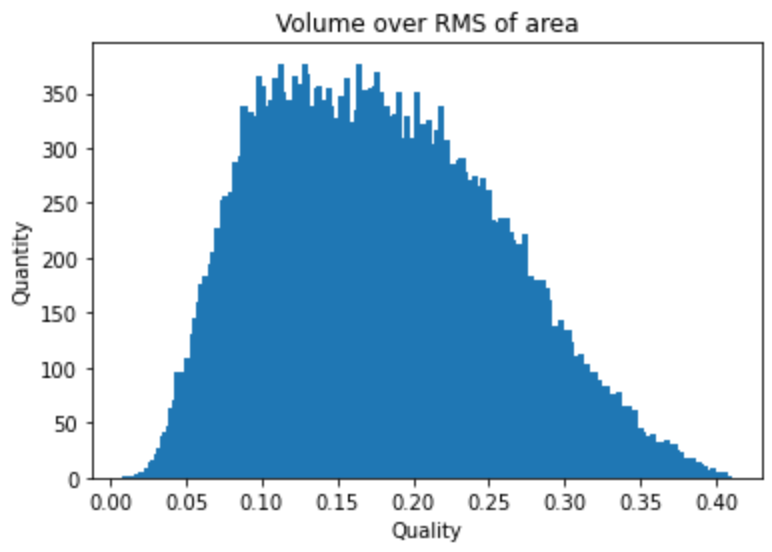
\includegraphics[width=\linewidth]{Materials/E1/voa1}
		\caption{Histogram of volume over RMS area measure.}
		\label{voa1}
	\end{subfigure}
	\\
	\begin{subfigure}[b]{0.49\linewidth}
		\centering
		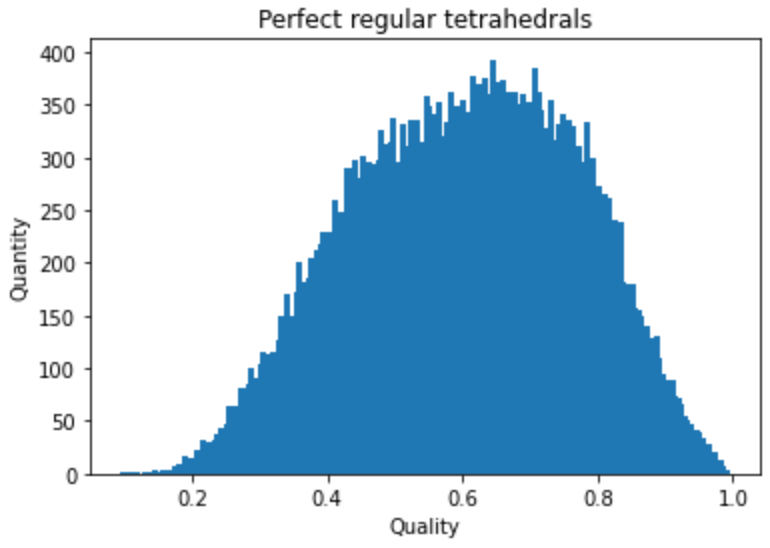
\includegraphics[width=\linewidth]{Materials/E1/pt1}
		\caption{Histogram of perfect tetrahedrals measure.}
		\label{pt1}
	\end{subfigure}
	\hfill
	\begin{subfigure}[b]{0.49\linewidth}
		\centering
		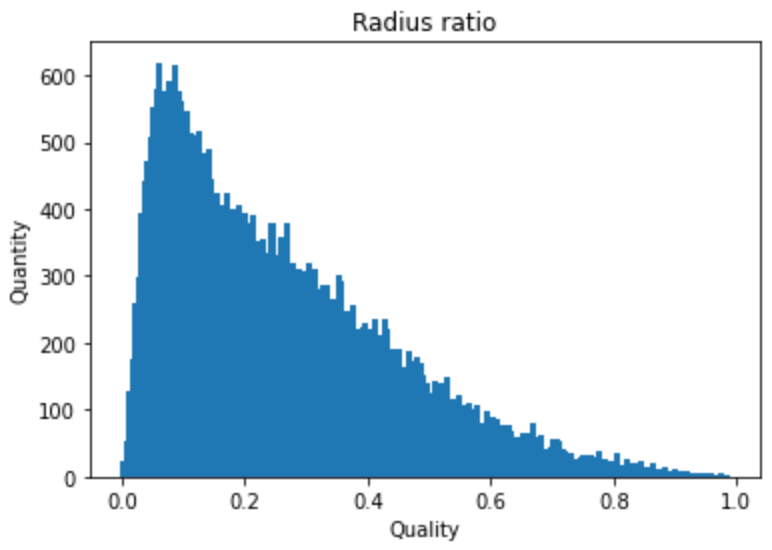
\includegraphics[width=\linewidth]{Materials/E1/rr1}
		\caption{Histogram of radius ratio measure.}
		\label{rr1}
	\end{subfigure}
	\caption{Histograms of quality measures for Armadillo tetrahedralized with \textit{stop\_quality} of 500.}
	\label{initial}
\end{figure} 
As we see, the quality of this mesh is rather poor, as there are no peaks in the histograms. This implies the tetrahedrals bein measured are not uniform which is what we would like them to be. More specifically we see from \autoref{pt1} that there are very few actual regular tetrahedrals, and the average value being around 0.6, implying quite poor optimal shape.\\
With this initial look at the tetrahedralized mesh, we would expect to be able to increase the mesh quality by decreasing the \textit{stop\_quality} parameter. The \textit{stop\_quality} adjusts how much AMIPS energy is tolerated in the mesh, which from Google searches seems to be a measure of distortion. This, when decreasing the amount of tolerated distortion in the mesh, we would expect the quality to rise. As it is not quite feasible to compare a range of histograms, we instead create box plots which can tell us about the spread or variance of the data and where the mean is. Using the Armadillo, we can now compute the tetrahedral mesh and perform the quality measure and plot the result as a box plot for \textit{stop\_quality} values in the range 50 to 1000. The results can be seen in \autoref{boxplots}.  
\begin{figure}
	\centering
	\begin{subfigure}[b]{0.49\linewidth}
		\centering
		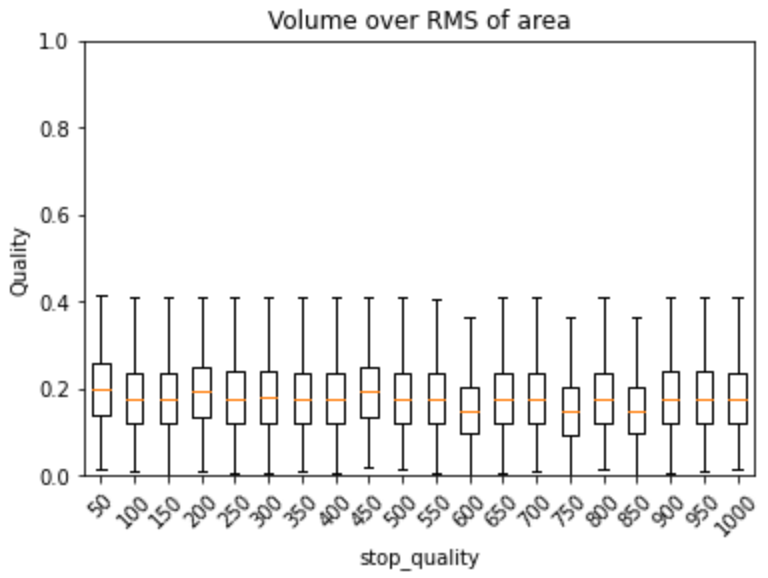
\includegraphics[width=\linewidth]{Materials/E1/voabox}
		\caption{Box plots of volume over RMS of area measures.}
		\label{voabox}
	\end{subfigure}
	\hfill
	\begin{subfigure}[b]{0.49\linewidth}
		\centering
		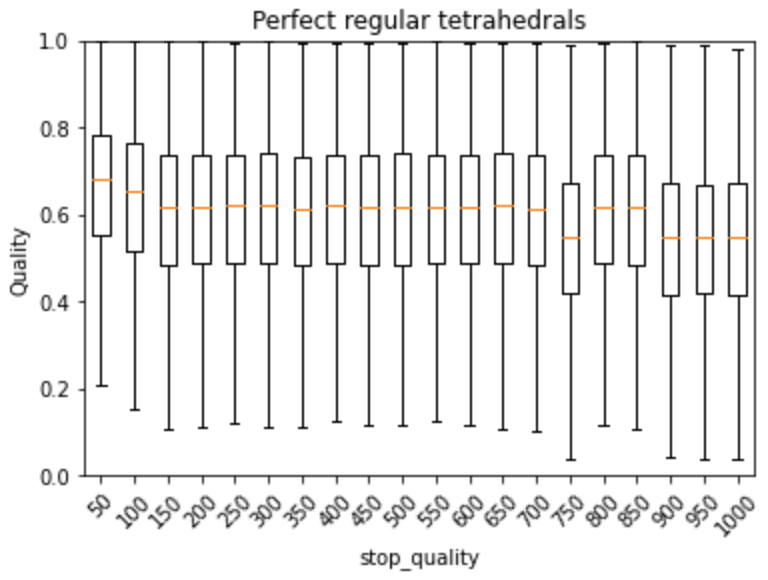
\includegraphics[width=\linewidth]{Materials/E1/ptbox}
		\caption{Box plots of perfect tetrahedrals measures.}
		\label{ptbox}
	\end{subfigure}
	\\
	\begin{subfigure}[b]{0.49\linewidth}
		\centering
		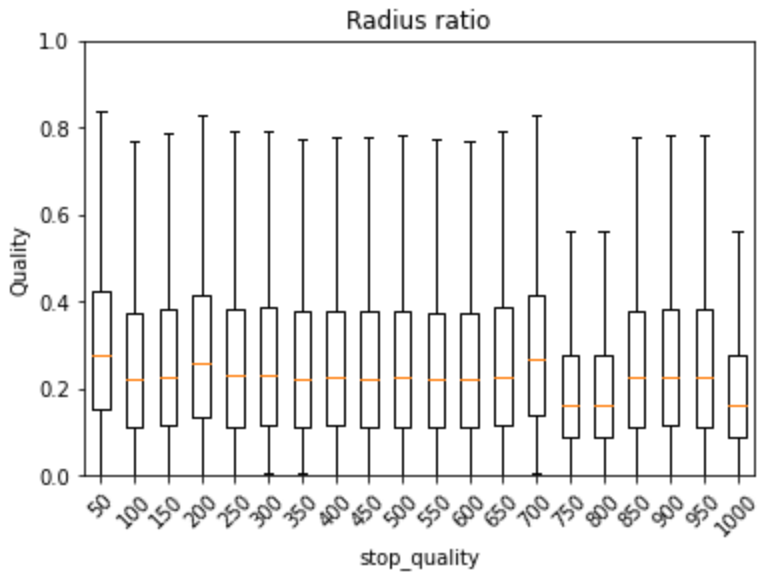
\includegraphics[width=\linewidth]{Materials/E1/rrbox}
		\caption{Box plots of radius ratio measures.}
		\label{rrbox}
	\end{subfigure}
	\caption{Box plots of quality measures for Armadillo mesh with \textit{stop\_quality} parameter setting in range 50 to 1000.}
	\label{boxplots}
\end{figure} 
In \autoref{voabox} we do not see too much change, but there seem to be a slight tendency for the variance to become smaller and smaller as \textit{stop\_quality} increases, however, the mean the data then centers around seem to be lower than at low \textit{stop\_quality} values. In \autoref{ptbox} we see a tendency of the mean getting lower as \textit{stop\_quality} increases, and the variance increasing as \textit{stop\_quality} increases. In \autoref{rrbox} we again seem to get quite similar results, but both the variance and mean of the data seem to shift downwards as \textit{stop\_quality} increases.
\subsection{Discussion of results}
We get a clear impression that the tetrahedrals become a lot more regular at lower \textit{stop\_quality} values as the mean is at the highest and the variance is at the lowest in \autoref{ptbox}. 
\begin{figure}
	\centering
	\begin{subfigure}[b]{0.49\linewidth}
		\centering
		\includegraphics[height=0.75\linewidth]{Materials/E1/Armadillo50}
		\caption{Armadillo tetrahedralized with \textit{stop\_quality} of 50.}
	\end{subfigure}
	\hfill
	\begin{subfigure}[b]{0.49\linewidth}
		\centering
		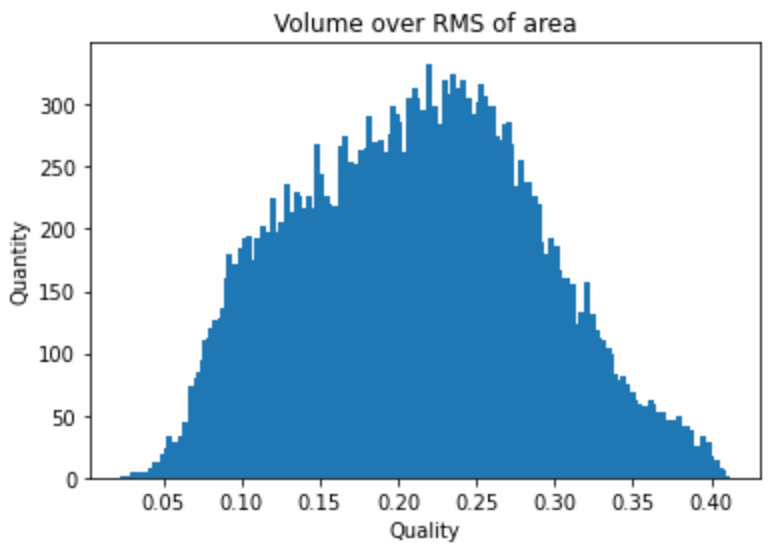
\includegraphics[width=\linewidth]{Materials/E1/voa2}
		\caption{Histogram of volume over RMS area measure.}
		\label{voa2}
	\end{subfigure}
	\\
	\begin{subfigure}[b]{0.49\linewidth}
		\centering
		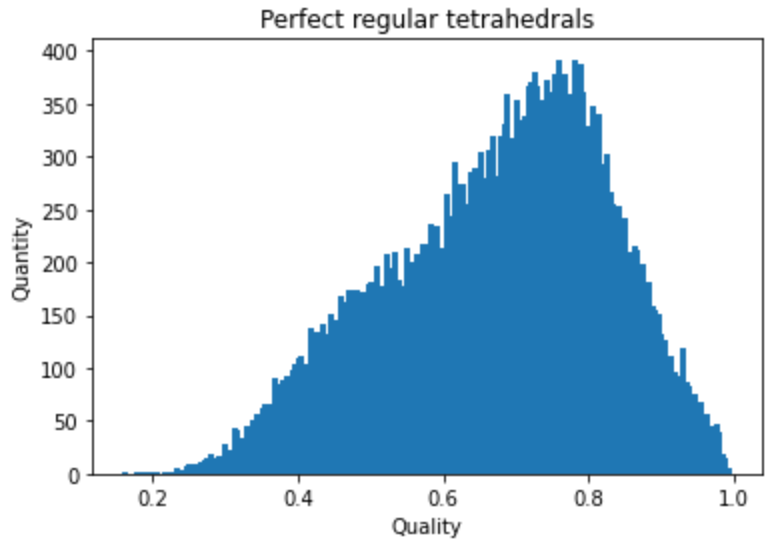
\includegraphics[width=\linewidth]{Materials/E1/pt2}
		\caption{Histogram of perfect tetrahedrals measure.}
		\label{pt2}
	\end{subfigure}
	\hfill
	\begin{subfigure}[b]{0.49\linewidth}
		\centering
		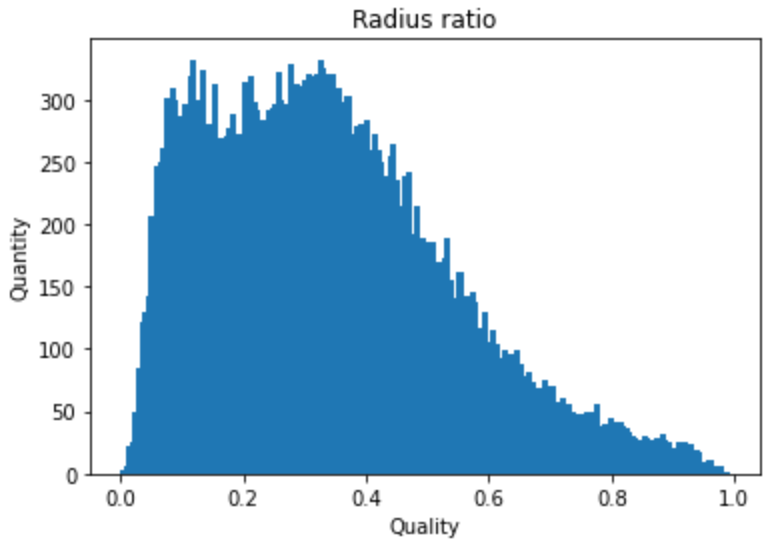
\includegraphics[width=\linewidth]{Materials/E1/rr2}
		\caption{Histogram of radius ratio measure.}
		\label{rr2}
	\end{subfigure}
	\caption{Histograms of quality measures for Armadillo tetrahedralized with \textit{stop\_quality} of 50.}
	\label{armadillo50}
\end{figure} 
However the box plots of the two other measures does not give a clear indication to a best \textit{stop\_quality} value. On one hand we want the quality to be the highest, and on the other we want the tetrahedrals to be uniform. As all three box plots agrees on the highest quality is found when \textit{stop\_quality} is low we choose to investigate this by plotting the histograms for the Armadillo with a \textit{stop\_quality} of 50 which can be seen in \autoref{armadillo50}. 
Comparing the two Armadillo meshes with the naked eye there is not too big of a difference, however, comparing the histograms in \autoref{initial} and \autoref{armadillo50} we see big improvements in the quality of the meshes. We see that the mean of the 'volume over RMS of area' has shifted up without the variances really changing, we see the variance has dropped a lot in 'perfect regular tetrahedrals' and the mean has shifted up, and finally we see the mean has shifted up for the 'radius ratio' although the variance has also increased quite a lot. We thus conclude that the quality can be improved by using lower \textit{stop\_quality} values when tetrahedralizing the Armadillo mesh. However, the variance or uniformity of the tetrahedrals suffer to some extend when it comes to the 'volume over RMS of area' measure and suffers quite a bit when it comes to 'radius ratio'. 

